\begin{frame}
\frametitle{Recognize speech, or, wreck a nice beach}
An automatic speech recognizers attempt to recognize the phrase
`recognize speech':

\begin{center}
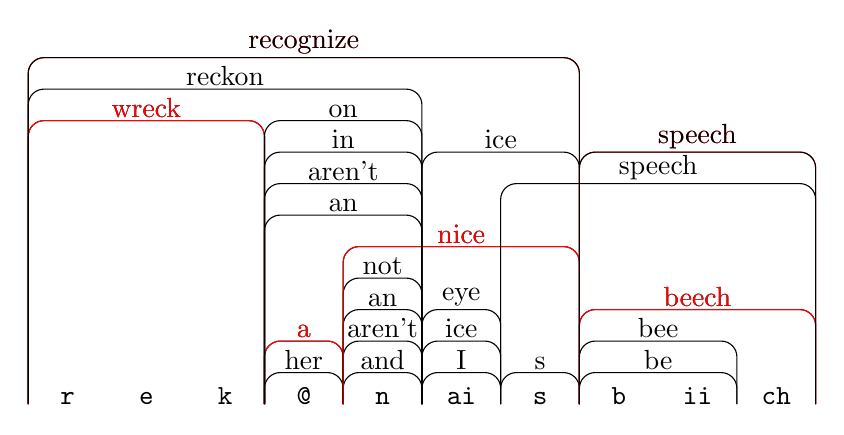
\begin{tikzpicture}[every node/.style={anchor=south,inner ysep=0.1em}]
\draw (0.5, 0)  node[anchor=base] {\texttt{r}};
\draw (1.5, 0)  node[anchor=base] {\texttt{e}};
\draw (2.5, 0)  node[anchor=base] {\texttt{k}};
\draw (3.5, 0)  node[anchor=base] {\texttt{@}};
\draw (4.5, 0)  node[anchor=base] {\texttt{n}};
\draw (5.5, 0)  node[anchor=base] {\texttt{ai}};
\draw (6.5, 0)  node[anchor=base] {\texttt{s}};
\draw (7.5, 0)  node[anchor=base] {\texttt{b}};
\draw (8.5, 0)  node[anchor=base] {\texttt{ii}};
\draw (9.5, 0)  node[anchor=base] {\texttt{ch}};

\pgfsetcornersarced{\pgfpoint{2mm}{2mm}}
\def\height{0.4}

\pgfmathsetmacro{\y}{1*\height}
\draw (3,0) -- (3,\y) -- node {her} (4,\y) -- (4,0);
\draw (4,0) -- (4,\y) -- node {and} (5,\y) -- (5,0);
\draw (5,0) -- (5,\y) -- node {I} (6,\y) -- (6,0);
\draw (6,0) -- (6,\y) -- node {s} (7,\y) -- (7,0);
\draw (7,0) -- (7,\y) -- node {be} (9,\y) -- (9,0);

\pgfmathsetmacro{\y}{2*\height}
\visible<-2>{
\draw (3,0) -- (3,\y) -- node {a} (4,\y) -- (4,0);
}
\visible<3>{
\draw[red] (3,0) -- (3,\y) -- node {a} (4,\y) -- (4,0);
}
\draw (4,0) -- (4,\y) -- node {aren't} (5,\y) -- (5,0);
\draw (5,0) -- (5,\y) -- node {ice} (6,\y) -- (6,0);
\draw (7,0) -- (7,\y) -- node {bee} (9,\y) -- (9,0);

\pgfmathsetmacro{\y}{3*\height}
\draw (4,0) -- (4,\y) -- node {an} (5,\y) -- (5,0);
\draw (5,0) -- (5,\y) -- node {eye} (6,\y) -- (6,0);
\visible<-2>{
\draw (7,0) -- (7,\y) -- node {beech} (10,\y) -- (10,0);
}
\visible<3>{
\draw[red] (7,0) -- (7,\y) -- node {beech} (10,\y) -- (10,0);
}

\pgfmathsetmacro{\y}{4*\height}
\draw (4,0) -- (4,\y) -- node {not} (5,\y) -- (5,0);

\pgfmathsetmacro{\y}{5*\height}
\visible<-2>{
\draw (4,0) -- (4,\y) -- node {nice} (7,\y) -- (7,0);
}
\visible<3>{
\draw[red] (4,0) -- (4,\y) -- node {nice} (7,\y) -- (7,0);
}

\pgfmathsetmacro{\y}{6*\height}
\draw (3,0) -- (3,\y) -- node {an} (5,\y) -- (5,0);

\pgfmathsetmacro{\y}{7*\height}
\draw (3,0) -- (3,\y) -- node {aren't} (5,\y) -- (5,0);
\draw (6,0) -- (6,\y) -- node {speech} (10,\y) -- (10,0);

\pgfmathsetmacro{\y}{8*\height}
\draw (3,0) -- (3,\y) -- node {in} (5,\y) -- (5,0);
\draw (5,0) -- (5,\y) -- node {ice} (7,\y) -- (7,0);
\visible<2>{
\draw[red] (7,0) -- (7,\y) -- node {speech} (10,\y) -- (10,0);
}
\visible<1,3->{
\draw (7,0) -- (7,\y) -- node {speech} (10,\y) -- (10,0);
}

\pgfmathsetmacro{\y}{9*\height}
\visible<-2>{
\draw (0,0) -- (0,\y) -- node {wreck} (3,\y) -- (3,0);
}
\visible<3>{
\draw[red] (0,0) -- (0,\y) -- node {wreck} (3,\y) -- (3,0);
}
\draw (3,0) -- (3,\y) -- node {on} (5,\y) -- (5,0);

\pgfmathsetmacro{\y}{10*\height}
\draw (0,0) -- (0,\y) -- node {reckon} (5,\y) -- (5,0);

\pgfmathsetmacro{\y}{11*\height}
\visible<2>{
\draw[red] (0,0) -- (0,\y) -- node {recognize} (7,\y) -- (7,0);
}
\visible<1,3->{
\draw (0,0) -- (0,\y) -- node {recognize} (7,\y) -- (7,0);
}


\end{tikzpicture}
\end{center}

%\begin{center}
%\uncover<2->{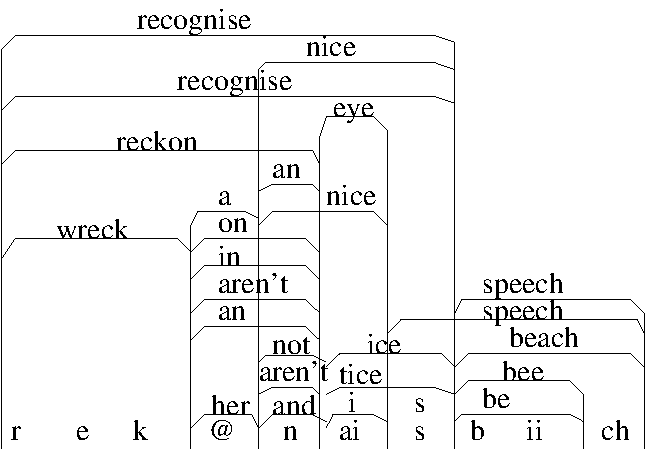
\includegraphics[height=0.5\textheight]{figures/rs1}}
%\end{center}
\tiny{$^*$Example reproduced from: (Shillcock, 1995)}
\end{frame}

\mode<article>{
NOTE: the total number of parses are 149, and there are another 100
paths from the start that ends with a dead end.
}
